\chapter{}\label{ex:aufg7}
%
\section{}\label{sec:aufg7a}
Die Ergebnisse der durchgeführten Messungen können in Abb. \ref{fig:Kennlinie_ohne_Korrektur} und Abb. \ref{fig:Kennlinie_mit_Korrektur} betrachtet werden.
\section{}\label{sec:aufg7b}
Der Unterschied, der Kennlinie bei kleinen Statorfrequenzen, der in Abb. \ref{fig:Kennlinie_ohne_Korrektur} gezeigt ist, liegt daran, dass der Statorwiderstand anders als angenommen bei ca. 25 $\Omega$ liegt und an diesem eine Spannung abfällt, wodurch nicht die gewünschte Spannung erreicht wird.
\section{}\label{sec:aufg7c}
Die Beziehung zwischen Statorstrombetrag $I_1$ und dem Statorwiderstand $R_1$ ergibt einen Spannungsabfall von:
\begin{equation}
	U = R_1 \cdot I_1
\end{equation}
Durch einen einfachen Regelkreis reagieren wir darauf mit einer Erhöhung der Spannung. 
\section{}\label{sec:aufg7d}
In Abb. \ref{fig:Kennlinie_ohne_Korrektur} kann man sehr leicht erkennen, dass das gewünschte Drehmoment aufgrund des Statorwiderstandes nicht erreicht werden kann. Durch die Korrekturmaßnahmen liegen die Kennlinien in Abb. \ref{fig:Kennlinie_mit_Korrektur} höher, allerdings nur vier der Kennlinien. Dies liegt daran, dass wir einen Spannungsabfall detektieren, und darauf mit einer Erhöhung der Spannung reagieren, dies funktioniert natürlich nur im Bereich zwischen 0 und 50 Hz, weil wir danach die Spannung nicht noch weiter erhöhen können.
\newpage
\begin{figure}[htb]
	\centering
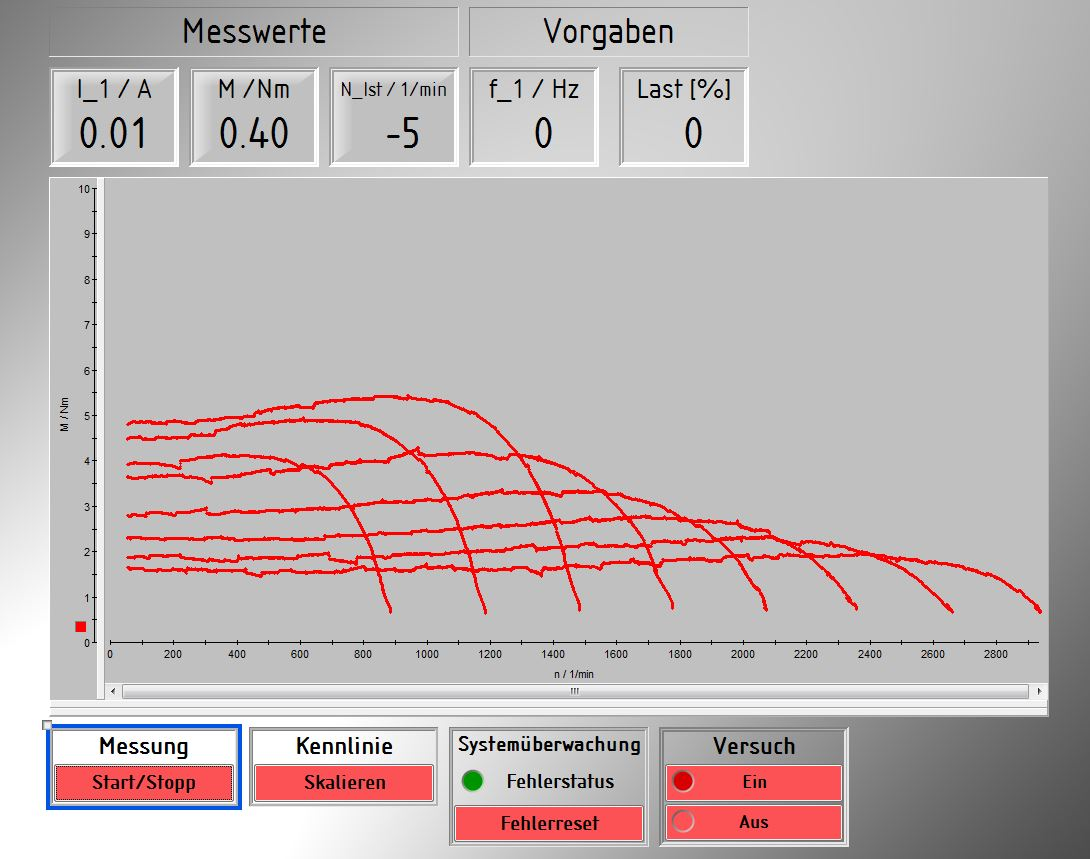
\includegraphics[width=0.8\textwidth]{./Bilder/Messung_Kennlinienfeld_ohne_Korrektur_A7}
\caption{Kennlinie ohne Korrektur}
\label{fig:Kennlinie_ohne_Korrektur}
\end{figure}
\begin{figure}[!htb]
	\centering
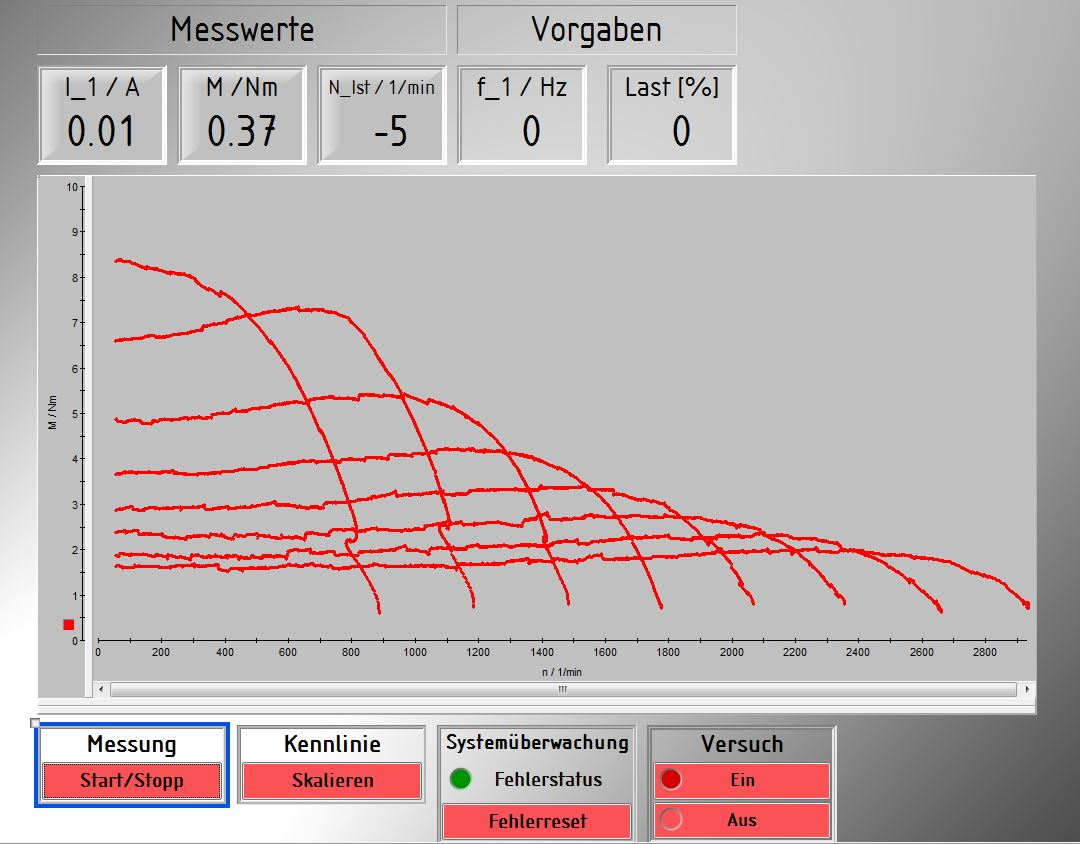
\includegraphics[width=0.8\textwidth]{./Bilder/Messung_Kennlinienfeld_mit_Korrektur_A7}
\caption{Kennlinie mit Korrektur}
\label{fig:Kennlinie_mit_Korrektur}
\end{figure}
